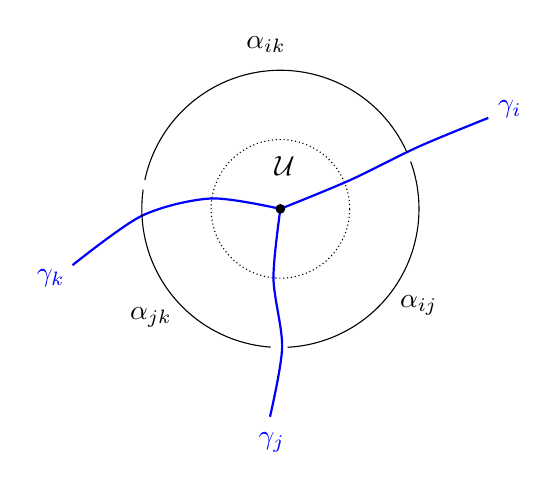
\begin{tikzpicture}[scale=1.1]
  \draw[densely dotted] (0,0) circle (0.8);
  \node at (0.05,0.5) {$\mathcal U$};
  % three arcs meeting at a vertex
  \draw[thick,blue] plot[smooth] coordinates {(0,0) (0.8,0.33) (1.6,0.72) (2.4,1.05)};
  \draw[thick,blue] plot[smooth] coordinates {(0,0) (-0.08,-0.8) (0.02,-1.6) (-0.12,-2.4)};
  \draw[thick,blue] plot[smooth] coordinates {(0,0) (-0.8,0.12) (-1.6,-0.08) (-2.4,-0.65)};
  \node[blue] at (2.65,1.15) {$\gamma_i$};
  \node[blue] at (-0.1,-2.7) {$\gamma_j$};
  \node[blue] at (-2.65,-0.8) {$\gamma_k$};
  % the three angles at the vertex
  \draw (24:1.6) arc (24:168:1.6);
  \node at (95:1.9) {$\alpha_{ik}$};
  \draw (-87:1.6) arc (-87:20:1.6);
  \node at (-35:1.95) {$\alpha_{ij}$};
  \draw (172:1.6) arc (172:266:1.6);
  \node at (220:1.95) {$\alpha_{jk}$};
  \fill (0,0) circle (1.6pt);
\end{tikzpicture}
